\chapter{Use cases for $2D$ Matching}

The chapter cover example of using MicMac when the matching problem is
a $2$ dimensionnal problem. This can occurs in the following situation :


\begin{itemize}
   \item the problem is intrinsiquely $2$ dimensionnal, for example in
         movement detection;

   \item the problem shoulde be $1$ dimensionnal, but the orientation parameters
         are unknown or, at least, unaccurate;
\end{itemize}

%-------------------------------------------------------------------
%-------------------------------------------------------------------
%-------------------------------------------------------------------


\section{The Mars data-set}



\begin{figure}
\begin{center}
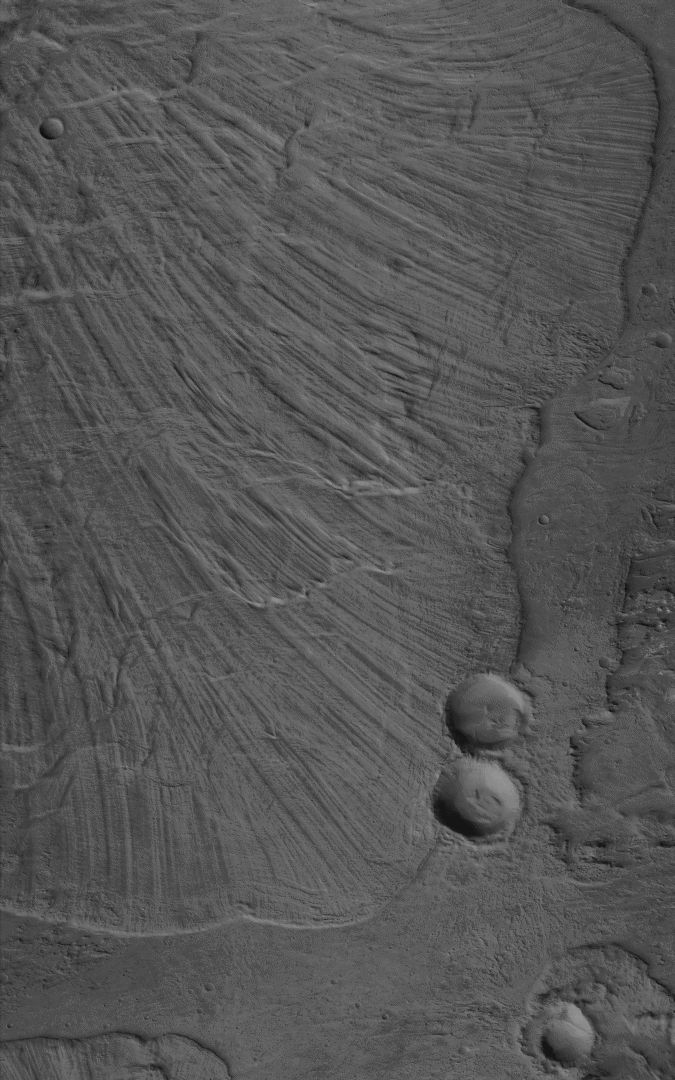
\includegraphics[width=35mm]{FIGS/Mars/SmaIm1.jpg}
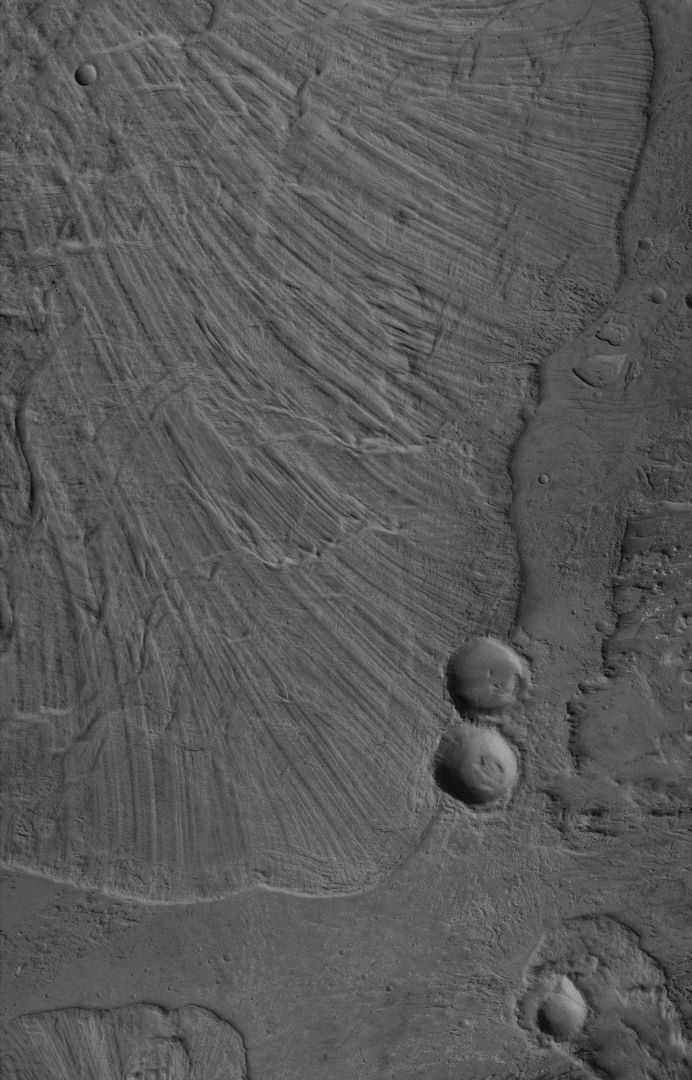
\includegraphics[width=35mm]{FIGS/Mars/SmIm2.jpg}
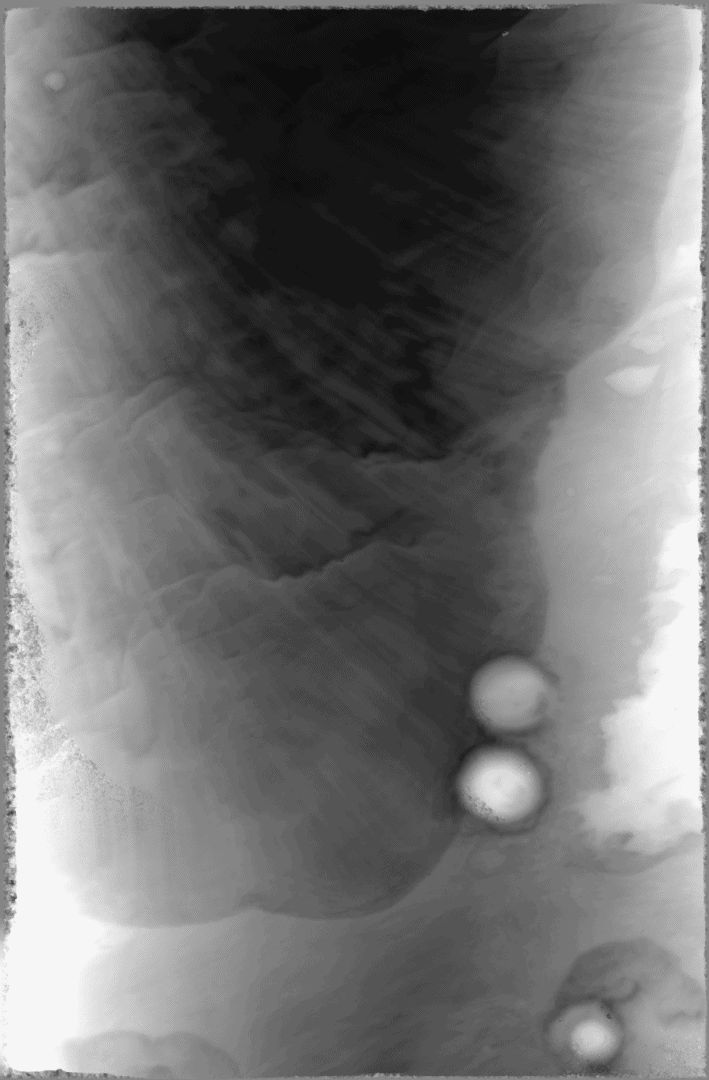
\includegraphics[width=35mm]{FIGS/Mars/Px1.jpg}
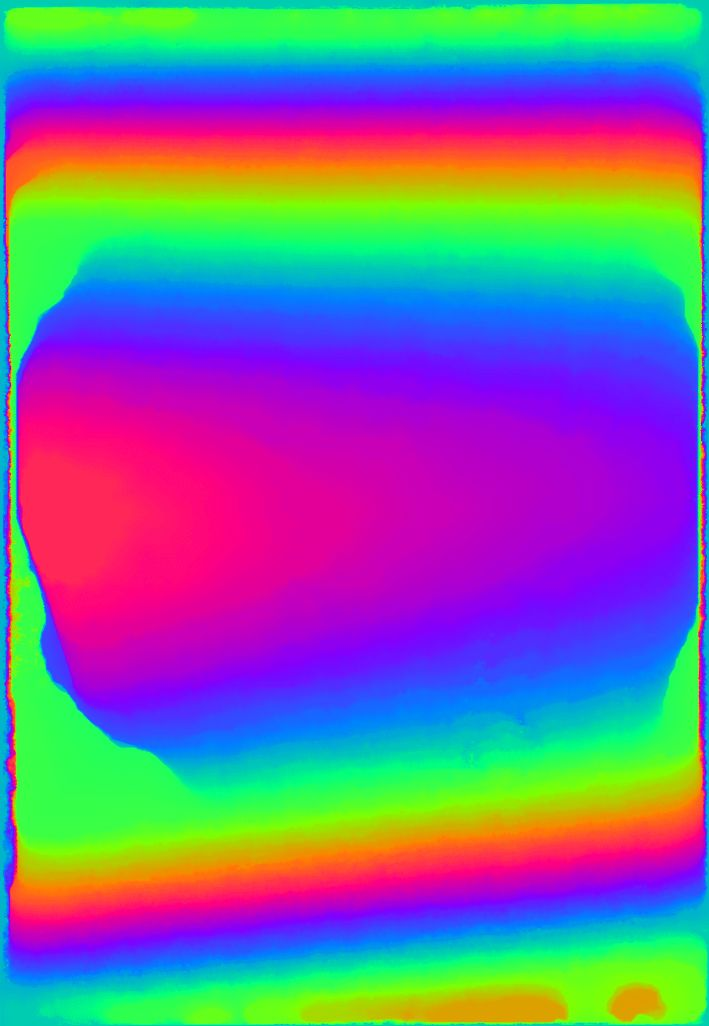
\includegraphics[width=35mm]{FIGS/Mars/Px2.jpg}

\end{center}
\caption{Mars data-set : the two  images, the $X$ paralaxe, in gray-level, and the $Y$-paralax in 
hue colour}
\label{FIG:OK:Mars}
\end{figure}

\subsection{Description of the data set}

The data can be found in directory {\tt Mars/} of directory {\tt ExempleDoc/}.
It consist of two stereo images acquired by Cassini (??) sond. In this case
we do not have the physicall model of the sensor, but we know that :

\begin{itemize}
   \item the satellite is a  pushbroom-satellite;
   \item it flights in the $x$ direction.
\end{itemize}

\subsection{Comment on the paramaters}

\subsubsection{Geometry}

The tags controlling geometry are :

\begin{itemize}

   \item   {\tt <GeomImages> eGeomImage\_Hom\_Px </GeomImages>} indicate the geometry of the acquisition,
          here it means that there is a principal homography $H$, let $P_1=x_1,y_1$ and  $P_2=x_2,y_2$ be two
          homologous points, MicMac will compute $U(P_1)$ and $V(P_1)$ such that

\begin{equation}
    P_2 = H(P_1) + (U(P_1),V(P_1))
\end{equation}

   \item  the homography $H$ is computed by MicMac from a set of homologous point;

   \item  {\tt  <FCND\_CalcHomFromI1I2> NKS-Assoc-CplIm2Hom@-Man@xml  </FCND\_CalcHomFromI1I2>}  indicates
          where {\tt MicMac} must look for the tie points (see directory {\tt Homol-Man/});


   \item  {\tt <GeomMNT> eGeomPxBiDim  </GeomMNT>} indicateseGeomImage the geoemtry of restitution,
          the value {\tt eGeomPxBiDim} indicate that what is copmuted is pixel offset, in fact this value
          is mandatory when using {\tt eGeomImage\_Hom\_Px}


\end{itemize}

\subsubsection{Matching}

In this case, the two paralax direction have completely different meanings :

\begin{itemize}
   \item the paralax $1$ represente mainly the relief, it is expected to contain high frequencies;
   \item the paralax $2$ represente mainly the error of the geometric model, it is expected to have
         low amplitude and low frequencies;
\end{itemize}

This dissymetry in \emph{a priori} knowledge on paralax is specified at different part of the file :

\begin{itemize}
   \item {\tt <Px1IncCalc>}   and {\tt <Px2IncCalc>},  representinng the global incertitude on each paralax;
   \item {\tt <Px1Regul>}   and {\tt <Px2Regul>},  representinng the \emph{a priori} knowledge on regularity of each
         paralax;
   \item {\tt <Px1PenteMax>}   and {\tt <Px2PenteMax>},  representinng the \emph{a priori} knowledge on the
         steep of each paralax;
   \item {\tt <Px1Pas>}   and {\tt <Px2Pas>},  representing the discretization step (as Px2 is low frequency and
         low amplitude, we can compute it with higher precision);
   \item {\tt <Px1DilatAlti>}   and {\tt <Px2DilatAlti>}, to gain som time, we decide not re-estimate Px2 at last step;
\end{itemize}

\subsubsection{Results}

Figure~\ref{FIG:OK:Mars} present the two images and the results of computed paralax.
As expected :

\begin{itemize}
   \item The Px1 contains mainly high frequency information on the relief;
   \item The Px2 contains mainly low frequency information on  geometry of the sensor.
\end{itemize}


%-------------------------------------------------------------------
%-------------------------------------------------------------------
%-------------------------------------------------------------------



\section{The Gulyia Seism data-set}
%-------------------------------------------------------------------

\subsection{Description of the data set}

The data can be found in directory {\tt SeismGuyla/} of directory {\tt ExempleDoc/}.
It consist of  two \emph{Spot 5} ortho photo of the same scen taken in $2002$ and
$2008$. Between these two dates, a seism occured and image matching can be used to
localize the break and quantify the movement.

We want to use MicMac to measure very fin displacement (arround $\frac{1}{10}$ pixel) in
a context where the image are quite different. Figure~\ref{FIG:OK:Guylia} present the two
ortho images.

\begin{figure}
\begin{center}
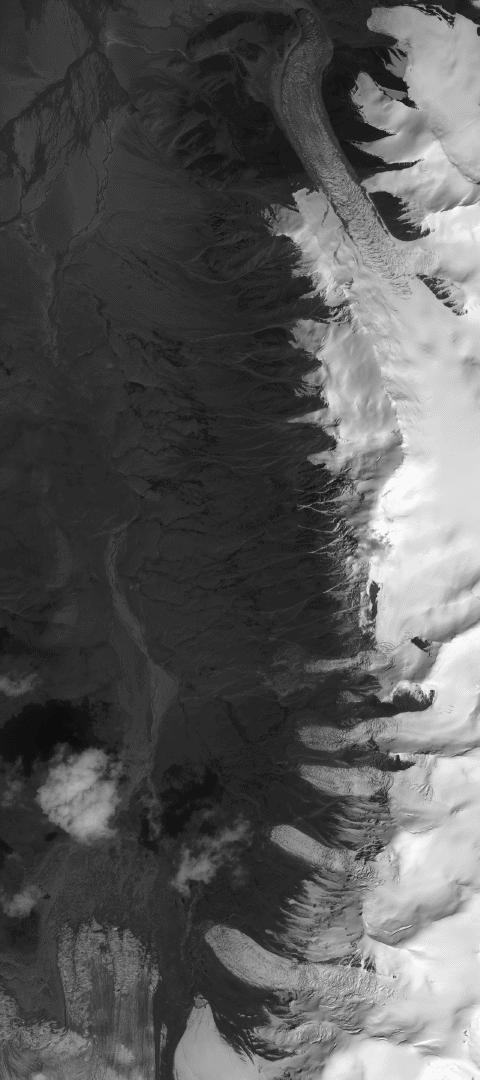
\includegraphics[width=35mm]{FIGS/SeismGuylia/250802_ortho.jpg}
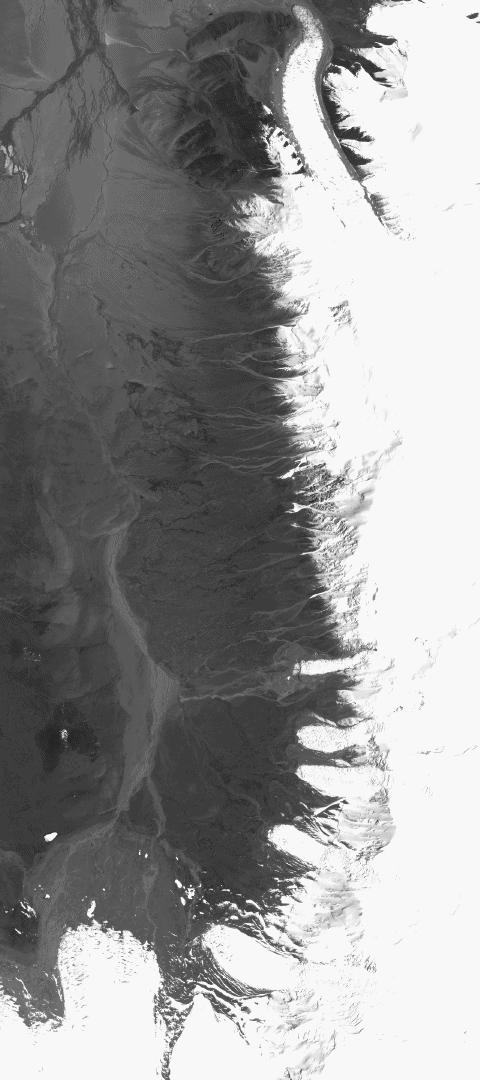
\includegraphics[width=35mm]{FIGS/SeismGuylia/260608_ortho.jpg}
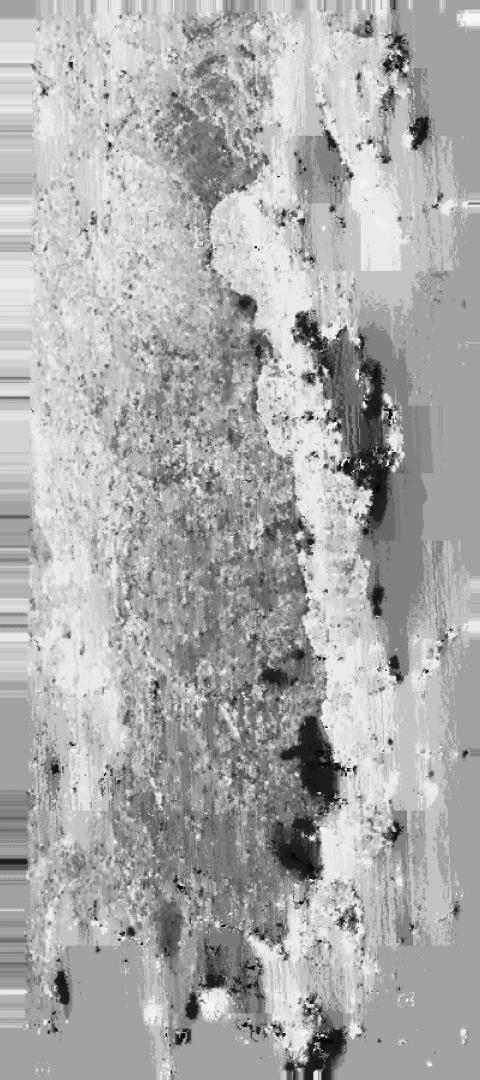
\includegraphics[width=35mm]{FIGS/SeismGuylia/Px1.jpg}
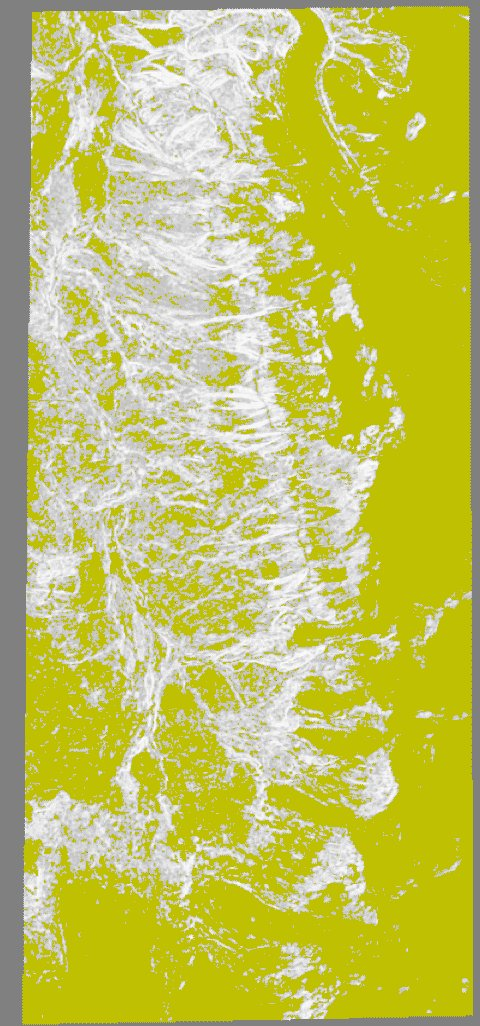
\includegraphics[width=35mm]{FIGS/SeismGuylia/Correl.jpg}

\end{center}
\caption{Guliya data set : the two ortho images, the $X$-paralaxed computed, and the correlation
coefficient computed}
\label{FIG:OK:Guylia}
\end{figure}




\subsection{Comment on the paramaters}


\subsubsection{Interpolation}

Aiming at measuring very fine displacment, we use a sinus cardinal interpolation :

\begin{itemize}
   \item {\tt <ModeInterpolation> eInterpolSinCard </ModeInterpolation>}

   \item  {\tt <SzSinCard>  5.0 </SzSinCard>} specifies the size of the kernel;

   \item  {\tt  <SzAppodSinCard>  5.0 </SzAppodSinCard>} controls the shape of the appodization
          window (the general shape is a Tukey window, when SzAppodSinCard=SzSinCard, it turns to be
          a Hamming window);
\end{itemize}


\subsubsection{Image term}

By default in MicMac, the image term is $1-Cor$ where $Cor$ is the normalized cross correlation
coefficient. In such data-set, where the is locally very important change, this can be not
adequate because when there is changes of nature (snow \dots)  the correlation has no 
signification and it is better to consider that there is no information.
Three paramaters are used here to control the meaning of correlation :


\begin{itemize}
   \item {\tt  <CorrelMin> }=$C^{min}$ ,  
         so  that correlation bellow $<C^{min}$ have no influence;
   \item {\tt  <GammaCorrel> }=$\gamma$  , higher ie $\gamma$ higher is the influence of correlation
         close to $1$;
   \item {\tt  <DynamiqueCorrel>=eCoeffGamma } to activate the previous one \dots
\end{itemize}

Following equations indicate how these parameters define the conversion from correlation to cost :

\begin{equation}
    C_1=Max(Cor,C^{min}) , 
\end{equation}

\begin{equation}
   C_2 = \frac{C_1 -C^{min}}{1-C^{min}}
\end{equation}

\begin{equation}
   C_3 = {C_2} ^\gamma
\end{equation}

\begin{equation}
   Cost  = (1-C_3) * (1-C^{min});
\end{equation}

On figure~\ref{FIG:OK:Guylia}, left image present the corremlation coefficients. The yellow value corresponds to the threshold value (here $<0?5$).


\subsubsection{Non isotropics regularization}

It can happen that we have \emph{a priori} knowledge for privilegiate some direction of regularization.
This can be done using in conjonction the following parameters of {\tt EtapeProgDyn}:

\begin{itemize}
   \item  {\tt  <NbDir>}=$N$  fixes the number of direction that will be explored;
   \item  {\tt  <Teta0>}=$\theta_0$  fixes the number of direction that will be explored;
   \item  the direction that will explored are $\alpha_k=\theta_0 + k\frac{\pi}{N} , k\in[0,N-1]$
   \item if the parameters  {\tt <Px1MultRegul>}=$V_1$ or {\tt <Px2MultRegul> } are used, then the value
         of regulalrization in direction  $\alpha_k$ is  mutiplied by $V_1[k]$ ($V_1$ is a vector);
\end{itemize}

In this example, we regularise more direction close to $\frac{\pi}{2}$, with a weight 
$\frac{1}{1+\frac{10}{N}*K}$




